\section{Применение средств автоматизированного проектирования \\
  при разработке устройства}

\subsection{Обоснование выбора пакетов прикладного программного обеспечения \\
  для моделирования и проектирования устройства}

Из-за приверженности к свободному программному обеспечению
~\cite{GNU-philosophy}, для создания проекта печатной платы была
выбрана САПР с открытым исходным кодом \textit{KiCAD}
~\cite{kicad-license}.

Такой выбор связан, этическими соображениями, которые, будучи
кратко сформулированы, звучат как:
Если пользователи не контролируют программу,
программа контролирует пользователей ~\cite{ufair-nonfree-programs}.

Другая причина выбора данной САПР при разработке,
используемый в ней, текстовой формат файлов,
при котором данные в документах САПР представлены
не иначе как Эс-Выражения (англ. \textit{S-Expressions})
~\cite{kicad-sexpr}.

В отличие от бинарных файлов,
используемых в \textit{Altium Designer},
файлы созданные при разработке печатной платы,
в \textit{KiCAD} за счёт их использования текста
возможно разместить в репозитории системы контроля версий
\textit{git}.

\textit{Git} это распределённая система контроля версий 
исходного кода \cite{git-dvcs}.

Из-за формата, файлы \textit{KiCAD} могут быть обработаны, как
исходный код.
Это даёт возможность удобной кооперации, при совместной работе.

Например в едином репозитории печатной платы, один конструктор в
соответствующем файле создаёт принципиальную схему устройства, а
другой в свою очередь, синхронизировав изменения в файле через
\textit{git}, используя готовую схему трассирует печатную плату.

Более того, используя, так называемый монорепозиторий, как подход
работы с \textit{git}, в одном репозитории можно содержать как
печатную плату, так и исходный код прошивки микроконтроллера,
используемый в ней.

\begin{figure}[H]
  \centering
  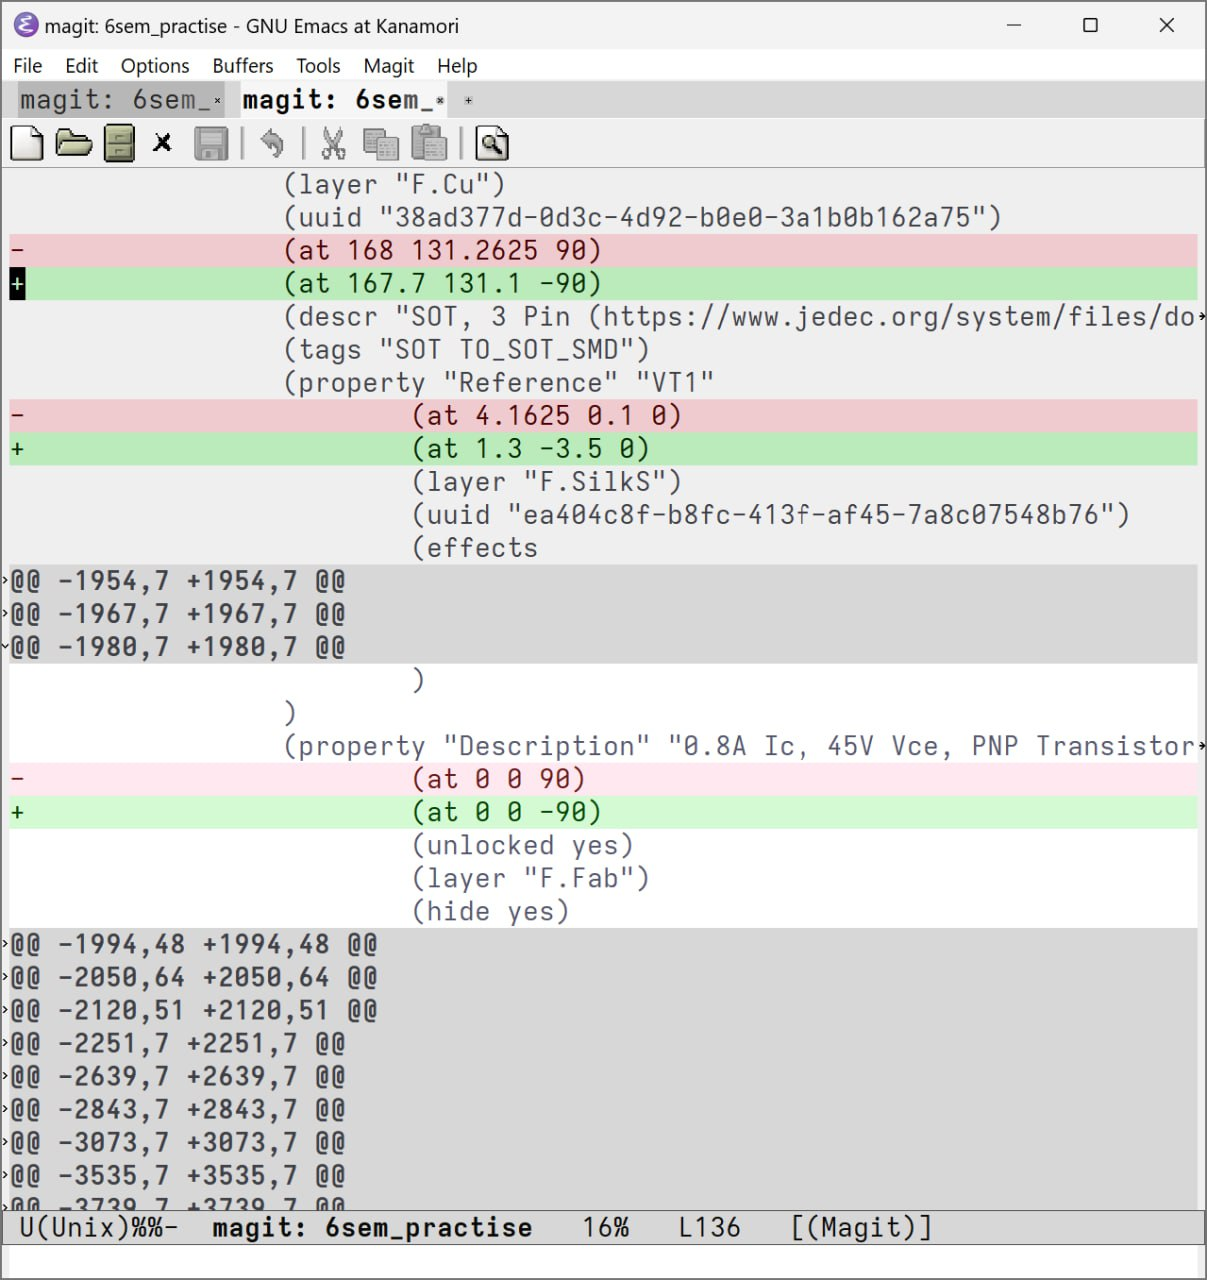
\includegraphics[scale=0.5]{magit-6-sem-practise.jpg}
  \caption{Снимок экрана с окном magit,
    установленный в расширяемый редактор текста GNU Emacs
    клиент системы контроля версий git.
    Видно, как magit может распознать изменения файла трассировки печатной платы,
    как добавление и удаление строк.}
\end{figure}

Для разработки печатной платы данного электронного модуля было
достаточно использование САПР ПП \textit{KiCAD}, однако стоит
отметить, что использование специальных САПР симуляторов,
например \textit{Proteus} или \textit{SimulIDE}
позволяет промоеделировать работу прицнипальной схемы,
используемой в ПП, а также получить информацию
нужную, например для вычисления коээфицента нагрузки устройства
$K_{\textrm{Н}}$ при расчете надёжности.

Для моделирования корпуса печатной платы использовался
трёхмерный параметрический САПР \textit{Компас 3D}.
Данная программа была выбрана ввиду доступности
её учебной версии, а также широким возможностям,
позволяющим конкурировать с программами
занимающими передовые места на рынке
трехмерных параметрических САПР.


\subsection{Технология применения средств автоматизированного проектирования \\
  при разработке конструкторской документации}

Большую сложность при выполнении работы составила необходимость
выполнять чертёж платы.
Интерфейс \textit{KiCAD-pcbdoc} рассчитан под трассировку печатной
платы, но никак не под черчение отдельного чертежа.
Присуствует возможность редактировать форматную рамку, наносить
разнообраные размеры, чертить на пользовательском слое.
Однако возможности выделить
каждый слой платы как отдельный вид нет.


%%% Local Variables:
%%% mode: LaTeX
%%% TeX-master: "main"
%%% End:
